\documentclass{beamer}

\usepackage[utf8]{inputenc}
\usefonttheme{professionalfonts}
\usepackage{tikz}
\usetikzlibrary{bayesnet}
\newcommand{\topline}{
  \tikz[remember picture, overlay] {
    \draw[gray, thick] ([xshift = 1cm, yshift = -1.2cm]current page.north west)
             -- ([xshift = -1cm, yshift = -1.2cm, xshift = \paperwidth]current page.north west);}}

\setbeamertemplate{frametitle}[default][center]
\setbeamertemplate{navigation symbols}{}
\setbeamerfont{footline}{series = \bfseries}
\setbeamertemplate{footline}[page number]

\begin{document}

\begin{frame}
\frametitle{\color{black}\textbf{Tensor Factorization}}
\topline
\footnotesize
{Bayesian treatment}\footnote{\scriptsize$\mathcal{N}(\cdot)$: Gaussian/Normal distribution; $\text{Gamma}(\cdot)$: Gamma distribution.}:
\vspace{-2em}
\begin{columns}
\begin{column}{0.6\textwidth}
\vspace{-15em}

\uncover<1->{\scriptsize{Suppose that \emph{the observation follows Gaussian distribution}:
\begin{equation*}
y_{ijt}\sim\mathcal{N}\left(\sum_{r=1}^{R}u_{ir}v_{jr}x_{tr},\tau^{-1}\right),(i,j,t)\in\Omega.
\end{equation*}
}
\uncover<2->{In the Bayesian setting, we place \emph{conjugate priors} on model parameters, i.e.,
\begin{equation*}
\begin{aligned}
\boldsymbol{u}_{i}&\sim\mathcal{N}\left(\boldsymbol{\mu}_{u},\Lambda_{u}^{-1}\right),i=1,2,\ldots,M, \\
\boldsymbol{v}_{j}&\sim\mathcal{N}\left(\boldsymbol{\mu}_{v},\Lambda_{v}^{-1}\right),j=1,2,\ldots,N, \\
\boldsymbol{x}_{t}&\sim\mathcal{N}\left(\boldsymbol{\mu}_{x},\Lambda_{x}^{-1}\right),t=1,2,\ldots,T, \\
\tau&\sim\text{Gamma}(\alpha,\beta). \\
\end{aligned}
\end{equation*}
}
}
\end{column}
\begin{column}[t]{0.35\textwidth}
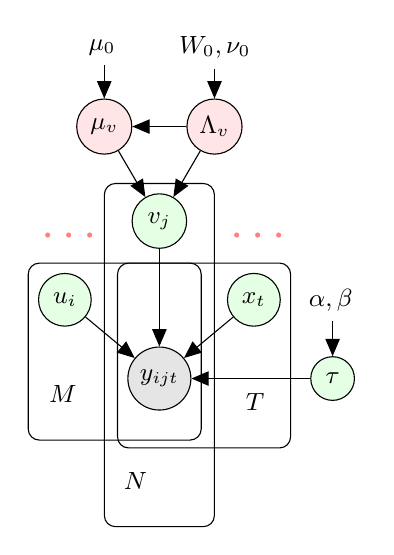
\begin{tikzpicture}
\uncover<1->{\node[circle,draw=black,fill=gray!20,inner sep=0pt,minimum size=0.8cm] (obs) at (2,-1) {\small{$y_{ijt}$}};
\node[circle,draw=black,fill=green!10] (ui) at (0.8,0) {\small{$\boldsymbol{u}_{i}$}};
\node[circle,draw=black,fill=green!10] (vj) at (2,1) {\small{$\boldsymbol{v}_{j}$}};
\node[circle,draw=black,fill=green!10] (xt) at (3.2,0) {\small{$\boldsymbol{x}_{t}$}};
\node[circle,draw=black,fill=green!10] (tau) at (4.2,-1) {\small{$\tau$}};
\path[draw=black,->] (ui) edge (obs);
\path[draw=black,->] (vj) edge (obs);
\path[draw=black,->] (xt) edge (obs);
\path[draw=black,->] (tau) edge (obs);
\node [text width=0.8cm] (m) at (1,-1.2) {\small{$M$}};
\plate[] {plate1} {(obs)(ui)(m)} { };
\node [text width=0.9cm] (n) at (2,-2.3) {\small{$N$}};
\plate[] {plate2} {(obs)(vj)(n)} { };
\node [text width=0.2cm] (f) at (3.2,-1.3) {\small{$T$}};
\plate[] {plate3} {(obs)(xt)(f)} { };
}
\uncover<2->{\node[circle,draw=black,fill=red!10,inner sep=0pt,minimum size=0.7cm] (muv) at (1.3,2.2) {\small{$\boldsymbol{\mu}_{v}$}};
\node[circle,draw=black,fill=red!10,inner sep=0pt,minimum size=0.7cm] (lambdav) at (2.7,2.2) {\small{$\Lambda_{v}$}};
\node[text width=0.6cm] (gamma) at (4.2,0) {\small{$\alpha,\beta$}};
\node[text width=0.4cm] (mu0) at (1.3,3.2) {\small{$\boldsymbol{\mu}_{0}$}};
\node[text width=0.9cm] (wnu0) at (2.7,3.2) {\small{$W_{0},\nu_{0}$}};
\node[text width=0.6cm] (cdots1) at (0.8,0.8) {\LARGE\color{red!50}{$\cdots$}};
\node[text width=0.6cm] (cdots2) at (3.2,0.8) {\LARGE\color{red!50}{$\cdots$}};
\path[draw=black,->] (muv) edge (vj);
\path[draw=black,->] (lambdav) edge (vj);
\path[draw=black,->] (lambdav) edge (muv);
\path[draw=black,->] (mu0) edge (muv);
\path[draw=black,->] (wnu0) edge (lambdav);
\path[draw=black,->] (gamma) edge (tau);
}
\end{tikzpicture}

\end{column}
\end{columns}

\end{frame}

\end{document}